%%%%%%%%%%%%%%%%%%%%%%%%%%%%%%%%%%%%%%%%%%%%%%%%%%%%%%%%%%%%%%%%%%%%%%
%% Copyright (c) 2016 Carsten Wulff Software, Norway
%% %%%%%%%%%%%%%%%%%%%%%%%%%%%%%%%%%%%%%%%%%%%%%%%%%%%%%%%%%%%%%%%%%%%
%% Created       : wulff at 2016-11-5
%% %%%%%%%%%%%%%%%%%%%%%%%%%%%%%%%%%%%%%%%%%%%%%%%%%%%%%%%%%%%%%%%%%%%
%% This program is free software: you can redistribute it and/or modify
%% it under the terms of the GNU General Public License as published by
%% the Free Software Foundation, either version 3 of the License, or
%% (at your option) any later version.
%%
%% This program is distributed in the hope that it will be useful,
%% but WITHOUT ANY WARRANTY; without even the implied warranty of
%% MERCHANTABILITY or FITNESS FOR A PARTICULAR PURPOSE.  See the
%% GNU General Public License for more details.
%%
%% You should have received a copy of the GNU General Public License
%% along with this program.  If not, see <http://www.gnu.org/licenses/>.
%%%%%%%%%%%%%%%%%%%%%%%%%%%%%%%%%%%%%%%%%%%%%%%%%%%%%%%%%%%%%%%%%%%%%%
%\documentclass[final,11pt]{IEEEtran}
\documentclass[crop,border=0pt]{standalone}
\usepackage{times}


%\usepackage{placeins}
\usepackage{upgreek}
\usepackage{amssymb,amsmath}
\usepackage{cite}
\usepackage{verbatim}
\usepackage{listings}
\usepackage{xcolor}
\usepackage{flafter}
\usepackage{booktabs}
\usepackage{url}
\usepackage{ textcomp }

\hyphenation{op-tical net-works semi-conduc-tor}


% -JSON styel

%\definecolor{darkGreen}{rgb}{0,0.2097,0}
%\newcommand{\myfigwidth}{\linewidth}
%\newcommand{\myfigwidtha}{\linewidth}
%\newcommand{\myfigwidthl}{\textwidth}
%\newcommand{\myfigwidthc}{0.6\linewidth}


\newcommand{\myfigwidtha}{3.3in}
\newcommand{\myfigwidthl}{7in}
\newcommand{\myfigwidthc}{2in}
%\newcommand{\myfigwidthe}{3.2in}
%\newcommand{\myfigwidthb}{5in}

\newcommand{\myfigname}{fig_}
\newcommand{\reg}[2]{{\figurename} \ref{#1}(#2)}
\newcommand{\req}[1]{{\figurename} \ref{#1}}
%\newcommand{\myeqname}{eq:}
%\newcommand{\req}[1]{(\ref{\myeqname#1})}

\definecolor{armygreen}{rgb}{0, 0.5, 0}
\newcommand{\missing}[1]{{ #1}}
\newcommand{\edit}[1]{{ #1}}
\newcommand{\secedit}[1]{{ #1}}
\newcommand{\deleted}[1]{{ #1}}
\newcommand{\moved}[1]{{ #1}}

%\newcommand{\missing}[1]{{\color{red} #1}}
%\newcommand{\edit}[1]{{\color{red} #1}}
%\newcommand{\secedit}[1]{{\color{armygreen} #1}}
%\newcommand{\deleted}[1]{{\color{violet} #1}}
%\newcommand{\moved}[1]{{\color{blue} #1}}

\newcommand{\SD}{Sigma-Delta }
\newcommand{\eqn}[1]{
  \begin{math}
    #1
  \end{math}}

\newcommand\JSONnumbervaluestyle{\color{blue}}
\newcommand\JSONstringvaluestyle{\color{red}}



\newif\ifcolonfoundonthisline

\makeatletter

\lstdefinestyle{json}
{
  showstringspaces    = false,
  keywords            = {false,true},
  alsoletter          = 0123456789.,
  morestring          = [s]{"}{"},
  stringstyle         = \ifcolonfoundonthisline\JSONstringvaluestyle\fi,
  MoreSelectCharTable =%
  \lst@DefSaveDef{`:}\colon@json{\processColon@json},
  basicstyle          = \fontsize{7}{7}\ttfamily,
  keywordstyle        = \fontsize{7}{7}\ttfamily\bfseries,
}

% flip the switch if a colon is found in Pmode
\newcommand\processColon@json{%
  \colon@json%
  \ifnum\lst@mode=\lst@Pmode%
  \global\colonfoundonthislinetrue%
  \fi
}

\lst@AddToHook{Output}{%
  \ifcolonfoundonthisline%
  \ifnum\lst@mode=\lst@Pmode%
  \def\lst@thestyle{\JSONnumbervaluestyle}%
  \fi
  \fi
  % override by keyword style if a keyword is detected!
  \lsthk@DetectKeywords%
}

% reset the switch at the end of line
\lst@AddToHook{EOL}%
{\global\colonfoundonthislinefalse}

\makeatother

% \lstset{  basicstyle=\tiny}

% \lstset{
% basicstyle=\fontsize{11}{13}\selectfont\ttfamily
% }


\lstset{language=Java}




%\usepackage[paperwidth=\maxdimen,paperheight=\maxdimen]{geometry}


\usepackage{tikz,pgfplots}
\usepackage{ifthen}
\usepackage{calc}
\usetikzlibrary{patterns}
%\usepackage[tightpage,active]{preview}
\usetikzlibrary{circuits.logic.US}
\usetikzlibrary{circuits.ee.IEC}
\usepgflibrary{shapes.arrows}
\usepgflibrary{arrows}
\usepackage{circuitikz}


% circuitikz draws bipole outlines (resistors, diodes, capacitors) at
% bipoles/thickness times the ambient line width, and the default is 2.
% That makes a circuitikz resistor visibly heavier than the wire it sits
% on, and heavier than the hand rolled zig-zag in ckt_lib.tex. One is the
% house width: everything is drawn at the environment's own thickness.
% Arrow tips: one filled tip everywhere, set through the '>' knob so a
% figure only ever writes ->, <- or <->. Latex (from arrows.meta)
% scales with the line width, so it stays in proportion if a drawing
% is ever set thicker or thinner than the house 'thick'.
\usetikzlibrary{arrows.meta}
\tikzset{>={Latex}}

\ctikzset{bipoles/thickness=1}
\ctikzset{tripoles/mos style/arrows}
\ctikzset{tripoles/pmos style/emptycircle}
%\PreviewEnvironment{circuitikz}
\pagestyle{empty}


\tikzstyle{cicfill}=[minimum size=1.4em]
\tikzstyle{stuff_fill}=[rectangle,fill=white,minimum size=1.4em]

\newcommand{\grayOne}{0.3 }
\newcommand{\grayTwo}{0.15 }
\newcommand{\grayThree}{0.26 }
\newcommand{\grayFour}{0.41 }
\newcommand{\grayFive}{0.61 }
\newcommand{\graySix}{0.85 }

%- Gray tone
%\definecolor{active}{rgb}{\graySix,\graySix,\graySix}
%\definecolor{poly}{rgb}{\grayFive,\grayFive,\grayFive}
%\definecolor{contact}{rgb}{\graySix,\graySix,\graySix}
%\definecolor{mOne}{rgb}{\grayFour,\grayFour,\grayFour}
%\definecolor{mTwo}{rgb}{\graySix,\graySix,\graySix}
%\definecolor{mThree}{rgb}{\grayThree,\grayThree,\grayThree}
%\definecolor{mFour}{rgb}{\grayTwo,\grayTwo,\grayTwo}

\definecolor{grey}{rgb}{1,1,1}
\definecolor{lightgrey}{rgb}{\grayFour,\grayFour,\grayFour}
\definecolor{active}{rgb}{0.4,1,0.6}
\definecolor{poly}{rgb}{1.0,0.5,0.5}
\definecolor{cut}{rgb}{0.91,0.91,0}
\definecolor{mOne}{rgb}{0.36,0.36,1}
\definecolor{mTwo}{rgb}{0.655,0.655,0}
\definecolor{mThree}{rgb}{0.3,1,1}
\definecolor{mFour}{rgb}{0,0.2097,0}
\begin{document}


% Spectrum of the GR06 reading over 120 minutes, as
% measured: only a straight line is removed from each segment, so the
% slow temperature drift rises below about 30 mHz. The dashed line is
% Machlup's Lorentzian for a 534 mK step with mean dwell
% times of 3.7 s and 1.4 s, not a fit: flat below
% 0.15 Hz, falling as 1/f^2 above. Above 1 Hz the reading has more
% than the trap, short visits the detector misses and the sensor's own
% noise.
%
% Generated by py/tikzplot.py. Edit the script in ex/ that
% produced it and re-run that, not this file.

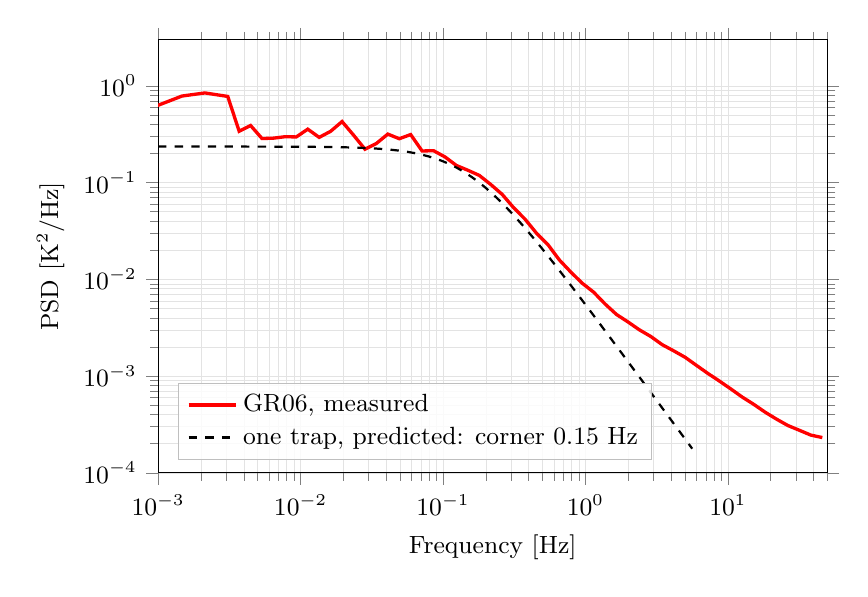
\begin{tikzpicture}[thick]

\begin{axis}[
  width=8.5cm,
  height=5.5cm,
  scale only axis,
  grid=both,
  grid style={gray!22, very thin},
  tick align=outside,
  tick label style={font=\small},
  label style={font=\small},
  title style={font=\small, yshift=-1mm},
  legend cell align=left,
  legend style={font=\small, draw=gray!50, fill=white, fill opacity=0.85, text opacity=1},
  xmode=log,
  ymode=log,
  xlabel={Frequency [Hz]},
  ylabel={PSD [K$^2$/Hz]},
  xmin=0.001,
  xmax=50,
  ymin=0.0001,
  ymax=3,
  legend pos=south west
]
\addplot[red, very thick, mark=none] coordinates {(0.0008453,0.5729) (0.001472,0.7859) (0.00213,0.846) (0.003083,0.7784) (0.003708,0.3399) (0.004461,0.3896) (0.005367,0.2855) (0.006457,0.2883) (0.007768,0.2983) (0.009345,0.2968) (0.01124,0.3572) (0.01352,0.2937) (0.01627,0.3394) (0.01957,0.4279) (0.02355,0.3099) (0.02833,0.2217) (0.03408,0.2539) (0.041,0.3176) (0.04932,0.2844) (0.05933,0.314) (0.07138,0.2124) (0.08587,0.2139) (0.1033,0.1844) (0.1243,0.1504) (0.1495,0.1343) (0.1799,0.1188) (0.2164,0.09576) (0.2603,0.07566) (0.3132,0.0551) (0.3768,0.04193) (0.4532,0.03004) (0.5453,0.02289) (0.656,0.01589) (0.7891,0.01192) (0.9494,0.009126) (1.142,0.007375) (1.374,0.005567) (1.653,0.004335) (1.989,0.003633) (2.392,0.003009) (2.878,0.002567) (3.462,0.002112) (4.165,0.001825) (5.011,0.001565) (6.028,0.001289) (7.252,0.001064) (8.724,0.0008884) (10.5,0.0007362) (12.63,0.0006064) (15.19,0.0005109) (18.27,0.0004236) (21.98,0.0003588) (26.45,0.0003079) (31.82,0.0002752) (38.28,0.0002454) (46.05,0.0002315)};
\addlegendentry{GR06, measured}
\addplot[black, thick, dashed, mark=none] coordinates {(0.001,0.2359) (0.001122,0.2359) (0.0012589,0.23589) (0.0014125,0.23589) (0.0015849,0.23588) (0.0017783,0.23588) (0.0019953,0.23587) (0.0022387,0.23586) (0.0025119,0.23585) (0.0028184,0.23583) (0.0031623,0.23581) (0.0035481,0.23578) (0.0039811,0.23575) (0.0044668,0.23571) (0.0050119,0.23566) (0.0056234,0.2356) (0.0063096,0.23551) (0.0070795,0.23541) (0.0079433,0.23529) (0.0089125,0.23512) (0.01,0.23492) (0.01122,0.23467) (0.012589,0.23435) (0.014125,0.23395) (0.015849,0.23345) (0.017783,0.23282) (0.019953,0.23203) (0.022387,0.23105) (0.025119,0.22982) (0.028184,0.2283) (0.031623,0.22641) (0.035481,0.22407) (0.039811,0.2212) (0.044668,0.21768) (0.050119,0.21341) (0.056234,0.20827) (0.063096,0.20214) (0.070795,0.19492) (0.079433,0.18652) (0.089125,0.17693) (0.1,0.16618) (0.1122,0.15436) (0.12589,0.14168) (0.14125,0.1284) (0.15849,0.11485) (0.17783,0.10138) (0.19953,0.088339) (0.22387,0.076025) (0.25119,0.064676) (0.28184,0.054444) (0.31623,0.045401) (0.35481,0.03755) (0.39811,0.030836) (0.44668,0.025171) (0.50119,0.020442) (0.56234,0.016533) (0.63096,0.013324) (0.70795,0.010708) (0.79433,0.0085861) (0.89125,0.0068716) (1,0.0054912) (1.122,0.0043828) (1.2589,0.0034947) (1.4125,0.0027845) (1.5849,0.0022172) (1.7783,0.0017646) (1.9953,0.0014038) (2.2387,0.0011164) (2.5119,0.00088769) (2.8184,0.00070566) (3.1623,0.00056087) (3.5481,0.00044573) (3.9811,0.0003542) (4.4668,0.00028144) (5.0119,0.00022361) (5.6234,0.00017765)};
\addlegendentry{one trap, predicted: corner 0.15 Hz}
\end{axis}

\end{tikzpicture}
\end{document}
